\section{Intellectual Merit of the Proposed Work}
\label{sec:future}

\subsection{Physics measurements at the CMS experiment at LHC}

The UNL HEP group plans a variety of physics measurements at CMS, matching the interests of group members, and covering an array of regimes where new physics might appear. The faculty and postdocs spearheading the physics topics discussed here all have past experience of CMS Run 1 and 2, and Tevatron experiments with the previous generations of most of these measurements. Such analyses will be further strengthened during the period of this award through synergistic interactions with the theorist Huang, a new faculty member at UNL, who has been funded by NSF to pursue research in LHC phenomenology, and who interacts closely with our experimental group.

\paragraph{Beyond observation: detailed studies of the Higgs sector} 
%%% General Higgs intro
So far, the  new 125~GeV boson has been found to match what is expected from the Higgs boson in the SM within experimental accuracy, including properties such as $J^P$ and couplings to fermions and bosons, as well as the modes of production and decay that are within reach of observations. As Higgs physics remains the centerpiece of the LHC physics program, the LHC experiments must delve deeper into this area of the SM and take the exploration beyond simple branching ratio measurements of the most probable decay modes and  the like. It is clear that the observed Higgs boson is involved in the electroweak symmetry breaking (EWSB), but is it the only player in it? What is the shape of the Higgs field potential? What is the CP structure of the coupling of Higgs to bosons and fermions? Does the observed Higgs boson couple to fermions of the first and second generation as expected? Each of these questions has critical importance for understanding the SM and may lead to observation of new phenomena. The UNL HEP group will work on several of these  topics, capitalizing on the expertise gained in multiple previous measurements with Higgs decays to vector bosons and Higgs production in associated with top.

%%% Hgg work that will be completed soon
Higgs decay to a pair of photons is one of the cleanest channels and one of the first seen at LHC. Our group is involved in multiple $H\to\gamma\gamma$ measurements that will be completed in the first half a year of this award. UNL postdoc Linda Finco is working on the cross section measurement of  $H\to\gamma\gamma$ with the full Run~2 dataset, which will be published by the end of 2019. Finco is also working on a search for another, low-mass, Higgs boson in the di-photon channel with the plan to submit a paper in the fall of 2019. In both of these, Finco is responsible for the online event selection and calibration of the trigger performance. Finco and graduate student Furong Yan expect to return to the baseline SM $H\to\gamma\gamma$ at the end of this award period, in 2021, once a year's worth of data is accumulated in Run~3.

%%% CP phases, CPV and anomamous couplings in H+jj via H->gamma gamma
% XXX Add references appropriately:
%   What is the reference for our tHq?
%   CP structure from H+jj: https://journals.aps.org/prl/pdf/10.1103/PhysRevLett.88.051801
%   CPV in Higgs SM and BSM: http://conferences.fnal.gov/win03/Talks/S%20Mrenna.pdf
%   Mention that we won't be sensitive to SM structure, but BSM detection is possible?
Couplings of the Higgs boson to fermions and vector bosons are its key properties, providing numerous observables for testing the SM.  Up until recently experimental efforts had focused on observing the production and decay modes and making first measurements of absolute coupling strengths. Our next target is examining the CP structure of Higgs couplings. SM sets the magnitude of the CP-even and odd phases in Higgs couplings to fermions and vector bosons, and predicts CP violation in Higgs production and decay. BSM theories, including SUSY, predict anomalous couplings or enhanced CP violation. The CMS physics program includes CP structure exploration for both fermion and vector boson couplings. The most sensitive method proposed to date involves the vector boson fusion production mode that yields a Higgs boson accompanied by two jets. The angular distributions of the Higgs and the jets provide a handle on the CP structure of the Higgs coupling to vector bosons. The two Higgs decays best suited for such study of $pp\to H+2$~jets are those to a pair of photons or $Z$ bosons. Capitalizing on the expertise of the UNL team, Kravchenko, a postdoc, and a future graduate student will lead the $H\to\gamma\gamma$ channel of the CPV and anomalous coupling search in the Higgs sector. The measurement will use the full Run~2 dataset.

The associated production of single top quarks with Higgs bosons is also sensitive to the CP structure of the Higgs couplings, as the production cross section has a strong dependence on the CP angle~\cite{bib:tH_theory}, with variations as large as an order of magnitude.  This was first explored in Monroy's dissertation~\cite{bib:monroy_thesis}. Bloom and Stieger will complete this measurement in the full Run~2 dataset, along with a measurement of the top-Higgs Yukawa coupling that follows up the measurement with 2016 data~\cite{bib:tHqRun2}.  That measurement shows some tension with the standard model, as a negative value of the coupling was only excluded with one standard deviation significance when four standard deviations was expected; the full dataset could help resolve this tension.  In addition, the new measurement will now be fully integrated with measurements of $t\bar{t}H$.  The $t\bar{t}H$ measurements will help constrain the magnitude of the coupling and provide more detailed information on the backgrounds to $tH$ production, and with this integration the $tH$ results will be included in the global fits over all Higgs production and decay modes to determine the Higgs couplings.  Bloom and collaborators are the only group in the U.S. on any LHC experiment working on this topic, with its unique abilities to probe the Yukawa coupling through Higgs production rather than decay.

%%% Di-Higgs production
The simplest Higgs potential of the SM that yields the observed EWSB is a purely theoretical conjecture. Mapping the true shape of the Higgs potential and measuring the Higgs boson self-couplings are already hot topics at LHC experiments, and are explored through studies of di-Higgs production. While the data collected are still far insufficient to observe Higgs pair production at the SM rates, CMS and ATLAS are already excluding BSM-predicted $HH$ production through spin-0 and spin-2 resonant states \cite{bib:radion-graviton-CMS,bib:radion-graviton-ATLAS} within a certain mass range, and in parts of non-SM couplings parameter space possible within EFT frameworks \cite{bib:HH-benchmarks}. Kravchenko and Kamalieddin are performing a resonant di-Higgs production measurement in which 
%one of the two produced Higgs bosons decays to a pair of $b$-quarks while the other decays to a pair of $Z$ bosons that subsequently decay to $\ell\ell\nu\nu$ final state in 2016 CMS data.
the $HH$ system decays as $HH\to bbZZ\to bb\ell\ell\nu\nu$ with the 2016 CMS data.
The combination of this channel with others will be published early fall 2019. Kravchenko and Finco, with collaborators, are starting an analysis with full Run~2 data where the $HH$ system decays to $bbZZ$ state and subsequently to all possible final states with leptons. To take the $HH$ measurements to the new sensitivity level, we rely on our expertise with the ongoing $HH$ search as well as in Finco's and Kravchenko's former $H\to ZZ$ and SM $Z$-boson production measurements. A new graduate student will join this effort.

% tHH version from Ken
%Just as single top-Higgs production provided unique information about the top-Higgs coupling, single top-double Higgs production provides unique information about the sign of Higgs self coupling.  As with the single Higgs case, the $tHH$ production rate is predicted to have a minimum at the SM value of the self coupling and increase by about an order of magnitude for negative coupling values, and in fact this variation is greater for $tHH$ than any other production mode~\cite{bib:HHproduction_theory}.  Limits on the production rate result in constraints on anomalous values of the self coupling.  Unfortunately, just as with single Higgs production,  SM $tHH$ production is expected to have a cross section several orders of magnitude below the dominant $gg$ fusion mode.  However, just as in Run~1, this mode is still worth exploring in case of anomalous effects.  Bloom, Stieger and a future student will explore this search, starting with multilepton final states, although $H \to b{\bar b}$ decays will probably also be required to gain reasonable sensitivity.

% tHH version from Ilya
Just as single top-Higgs production provided unique information about the top-Higgs coupling, single top-double Higgs production provides unique information about the sign of Higgs self coupling.  As with $tH$, the $tHH$ production rate is predicted to have a minimum at the SM self coupling value and increase by an order of magnitude for negative coupling values, with the rate variation for $tHH$ greater than for any other production mode~\cite{bib:HHproduction_theory}. While SM $tHH$ production is expected to have a cross section several orders of magnitude below the dominant gluon-fusion mode of $HH$ production, the enhancement due to negative or otherwise anomalous self coupling values can boost the rate dramatically. Setting limits on the production rates will result in constraints on values of the self coupling that are uniquely sign-sensitive. Bloom, Stieger and a future student will explore this topic, starting with multilepton final states, and adding $H \to b{\bar b}$ to gain sensitivity.

%KB took this out because it's stated in the EGM section.

%In addition to the exercise with Higgs measurements, and $Z$ boson and photon detection, our group is strongly involved with electron and photon reconstruction and identification, as well as with triggering on these objects, as discussed below. The  program of Higgs measurements involving diphoton and multilepton signatures is thus ideally suited to the strengths of our group.

\paragraph{Top physics}
%

%%% 4-top production
%   Add references:
%     - take a prediction, e.g. 13 TeV, from slide 5 of https://www.dropbox.com/s/ck1ml76nxskaats/4top_TopicOfTheWeek_28Nov17.pdf?dl=0
%     - quote Higgs width sensitivity from slide 7 of the above
In the past, the UNL group worked on many measurements of single and pair top quark production. With the large dataset of Run~2 it became possible to look for four-top production. The process $pp\to t\overline{t}t\overline{t}$ offers qualitatively new insights into SM physics processes and may be enhanced by new physics. This is a higher-order QCD production process with a difficult SM calculation due to many diagrams interfering; a measurement would help test theory predictions. Additionally, one can constrain Higgs width by comparing $ttH$ (a measurement in which UNL is involved) and $t\overline{t}t\overline{t}$ \cite{bib:Higgs-width-tttt}. Finally, supersymmetric, quark-composite, 2HDM and many other models predict modified production of $t\overline{t}t\overline{t}$. Fangmeier, advised by Snow and Golf, plan to continue working on this topic. Early results will be shown in mid-2019, while the full Run~2 measurements with multiple channels combined is expected to be published in 2020.

When Run~3 begins in 2021, the LHC is expected to operate at $\sqrt{s} = 14$~\TeV, and the CMS detector will have undergone a number of improvements.  It will be necessary both to recommission the detector and to make all the baseline SM measurements at the collision energy.  The $t\bar{t}$ system is a very natural place to do this, as it is so critical to understanding the SM and also as a background to BSM searches.  Bloom and postdocs and students collaborating with him will work in this area at the start of Run~3.

\paragraph{Standard model precision measurements}
%%% Drell-Yan measurements
%  Add references:
%     - ATLAS 3D DY cross section
Many SM precision measurements are possible with the vast Run~2 dataset, and the UNL group authored such results on vector boson and Higgs production. Kravchenko, a coordinator and main author of differential cross sections of the Drell-Yan process at 7, 8, and early 13~TeV data, will continue this line of research. With Drell-Yan measurements we can test perturbative QCD predictions at NNLO where the theory has recently rapidly developed thanks to LHC results, provide input to proton PDF fits at lower $x$ and higher $Q^2$, and compute the value of the weak mixing angle $\theta_w$, a fundamental electroweak observable. 
%Accurate understanding of Drell-Yan production is also critical for estimation of backgrounds to many Higgs and top physics measurements. 
Kravchenko and graduate student Robert Tabb are now working on the double differential Drell-Yan cross section with respect to invariant mass and rapidity of the mediating $Z/\gamma^*$ in the 2016-17 CMS dataset, with a paper expected to be submitted in early 2020. The next goal for Kravchenko and Tabb will be an ambitious measurement not yet been done in CMS but published by ATLAS \cite{bib:ATLAS-3D}: the differential Drell-Yan cross section with respect to the dilepton mass, rapidity, and leptonic decay angle in the Collins-Soper frame $\theta^*_{CS}$. In precision measurements, constraints on proton PDFs are limited by uncertainty on the value of $\theta_w$, while the measurements of $\theta_w$ are limited by PDF uncertainties. This unique 3D measurement allows theorists to dramatically reduce systematic uncertainty in simultaneous extraction of the $\theta_w$ and constraining the PDFs. The measurement will be performed with partners from Korea and Lithuania by the end of 2021. In Run~3, LHC will operate at an increased 14~TeV collision energy, cross sections of SM processes will be different and new regions of the Bjorken scaling variable and the evolution scale will become accessible. Beginning of 2022, Kravchenko and a future graduate student will analyze the first Run~3 data and measure the inclusive $Z$ production cross section and the differential Drell-Yan cross section with respect to the dilepton invariant mass.

% XXX Dan, please review here, W'/Z' content? Antyhing else?
\paragraph{Exotic phenomena beyond the standard model}
 Vector-like quarks appear in many new physics scenarios (composite higgs and little higgs models, SUSY extensions). They offer potential ways to avoid the hierarchy problem and explain the observed mass of the Higgs boson.  The pair-production of such quarks have been extensively searched for and in the absence of evidence of new physics are currently constrained to be around the TeV scale.  Without an increase in beam energy, progress slowed, necessitating new approaches. One promising strategy is to search for single production of vector-like quarks, the smaller $\alpha_{weak}$ coupling may be offset by a gain in the pdfs from smaller $\sqrt{\hat{s}}$. Single production may occur in either non-resonant or resonant production modes.  Recent results have begun to probe the non-resonant scenarios. Under Claes’ supervision graduate student Joaquin Siado Castenada is exploring these production modes in single lepton final states. In the context of this work, they will investigate modes of resonant production. As an interesting class, these new physics scenarios may also provide additional vector resonances (e.g. W’) that may have evaded current searches if they have large branching ratios to final states containing one or more vector-like quarks. The plan is to develop the analysis through 2018.

\subsection{Reconstruction, calibrations, software development, and offline computing}

\paragraph{Computing} The UNL HEP group will continue its operational responsibility for the U.S. CMS Tier-2 computing center, building on the established record of success in both operations and development. Bloom oversees expansions and upgrades of the computing cluster in accordance with CMS needs and the commitments of U.S. CMS to the Worldwide LHC Computing Grid.

Bloom and Stieger will continue their efforts to develop and improve the monitoring systems for CMS computing, taking advantage of the MONIT framework that is becoming the standard for all LHC experiments.  The job dashboard is now in a commissioning phase, and the production workflow infrastructure monitoring system is moving along.  Future targets include improved monitoring of data movement through the AAA system and the progress of individual tasks within the production system.  The validation of such monitoring is a good project for students who wish to build up experience with computing but do not start with a strong background.

Bloom will continue in a leadership role for the U.S. CMS Software and Computing Operations Program.  He will keep responsibility for the \$16M annual budget of the program, which funds the purchase of hardware at Fermilab's Tier-1 facility and the seven U.S. CMS HEP Tier-2 facilities and supports about 55~FTE computing experts who operate the facilities, develop and maintain critical pieces of the software and computing tools such as the data management and workflow management systems and the processing software framework, and pursue targeted research and development efforts to prepare CMS software and computing for future technologies.  This role requires day-to-day interaction with CMS software computing leaders, the CMS software and computing team based at Fermilab, leaders of the Operations Program, and the funding agencies.  Bloom receives partial support from the Operations Program for this work.

The Operations Program is strengthening its focus on the software and computing needs for the HL-LHC program.  Trigger rates could increase by as much as an order of magnitude, resulting in datasets that cannot be processed and analyzed under flat computing budgets without significant innovations.  In addition, the world of computing is moving into a period of rapid change and complexity.  The dominance of the x86 architecture has allowed for the establishment of standardized computing facilities that have been assembled into a worldwide computing grid, and particle physicists made great use of this homogeneity to facilitate scientific computing.  Future growth in computing capacity is expected to be based around accelerators such as GPUs and tensor processing units which will require a different kind of coding.  Further, these will be available through HPC centers  not designed with HEP use in mind.  A significant R\&D effort will be needed to make the best use of this new ecosystem.  Bloom will make progress in this area through his long-time collaborations with computer scientists such as Brian Bockelman, the co-PI of the new NSF-funded IRIS-HEP software institute.  A likely target is the area of data organization, access, management and access, and the expansion of the AAA data federation (started at UNL) into a U.S. ``data lake'' that will allow POSIX-like interfaces to the federation, add caching to minimize the impact of latency, and minimize the cost of on-disk copies of data.  Bloom will coordinate the rollout of data lake features across the U.S. CMS Tier-2 sites and then, if successful, to the CMS collaboration as a whole.  This R\&D work will help prepare CMS to submit its HL-LHC computing TDR in 2022.

\paragraph{Electron and photon objects}
Accurate reconstruction and identification of leptons and photons offline and at the trigger level drives the quality of CMS physics measurements. The experiment's Physics Object Groups (POG) develop reconstruction for these objects, calibrate physics observables, and provide  physics analysis teams  with guidance and recipes. POG conveners also ensure that each published measurement follows the prescribed usage of the objects. 

The EGM POG oversees everything related to electrons and photons in CMS, and was a major contributor to the Higgs discovery and subsequent measurements of Higgs properties, as Higgs searches rely on leptonic and photonic signatures. Kravchenko, Finco, and Fangmeier are presently involved in several activities of the EGM related to reconstruction, identification, and triggering.

%%% Ilya: this paragraph is shortened to save space
Kravchenko has served as a co-convener of the EGM Electron and Photon Identification subgroup, and had major responsibilities as a developer of the ID framework. 
%Each year there are multiple cycles of ID preparation for use in  CMS analyses with electrons and photons that involve tuning of the selection criteria, understanding differences in data and simulation, and producing efficiency scale factors for all ID packages. 
Kravchenko will continue being as an advising expert to the EGM team during ID development for ``ultra-legacy'' reconstruction of Run~2 data (2019) and first ID development for early Run~3 data (late 2021), at a light involvement level that would allow him to mainly focus on the Phase~2 projects described below.

%%% Ilya: This is a good passage, but we remove it to reduce the text size and
%%% to avoid over-commmitting me. 
%Kravchenko will continue coordinating Fangmeier's work on electron object reconstruction. The present project of electron track seeding development will be completed early in the period of this proposal. This will be followed by contributing to a significant electron reconstruction code revision in EGM in during the long shutdown, a convenient point to clean up and restructure the code.

The main focus of UNL activities in EGM will be in the trigger area. Finco has been appointed as a co-convener of the EGM HLT subgroup and brings extensive trigger experience as she was responsible for the trigger studies in several $H\to\gamma\gamma$ measurements and worked with photon triggers in the CMS Trigger Studies Group. She will coordinate the group in the next several years, and will lead major trigger code revisions and preparation of Run~3 EGM triggers.

The EGM part of the research plan provides our group with expertise and close involvement on all aspects related to electrons and photons, which significantly strengthens our effort of data analysis as most of our physics program involves multilepton and photon signatures.


\subsection{CMS Phase~2 upgrade}

%XXX Add the Phase~2 funding status with NSF and any TDR/FDR status info

The original CMS detector was designed to operate at a nominal LHC luminosity of $1\!\times\! 10^{34}\textrm{ cm}^{-2}\textrm{s}^{-1}$, with 25 proton-proton interactions (``pileup'') per bunch crossing. These conditions were achieved during Run~1 and surpassed in Run~2 with the luminosity increased by $\times$2 and pileup of 60, with Run~3 expected to be similar. A dramatic change is planned for Run~4 that opens the HL-LHC era in 2026, when luminosity will increase to $5\!\times\! 10^{34}\textrm{ cm}^{-2}\textrm{s}^{-1}$. To maintain and improve detector performance in the presence of radiation damage and growing number of pileup interactions, CMS undergoes periodic upgrades, starting with the Phase~1 upgrade in the long shutdown of LHC between Runs~1 and~2. The Phase~2 upgrade is planned for the long shutdown in 2024-26. Each upgrade involves major hardware changes or a full subdetector replacement and, thus, requires significant time and resources, years of R\&D, and then construction of detector components, to be ready for installation by the start of a long shutdown.

The pixel detector sits closest to the interaction region and is crucial for the charged particle track reconstruction that underpins nearly all CMS physics analyses. The UNL HEP group has played a major role in the design, construction, installation and operation of the original CMS Pixel Detector, and was one of the leading institutions in executing the Phase~1 upgrade. The UNL HEP group contribution is discussed in detail in Section~\ref{sec:prior}. 

In the Phase~2 upgrade, the full CMS tracking system will be replaced with a new Outer and Inner Tracker\cite{bib:Phase2TDR}. The design and construction of the TFPX portion of the Inner Tracker (Fig.~\ref{fig:TFPX}) is a U.S.~CMS responsibility and the flagship of the upcoming NSF MREFC upgrade project.  The TFPX is conceptually similar to the Pixel Detector: it is based on silicon modules with fine pixelated sensors and readout chips. The technology choices and electronics design reflect more demanding operating conditions, and the tracking coverage is extended from pseudorapidity up to 2.5 (present) to 4.0 (Fig.~\ref{fig:TFPX}), significantly enhancing the physics potential of the detector. 


\begin{figure}
\centering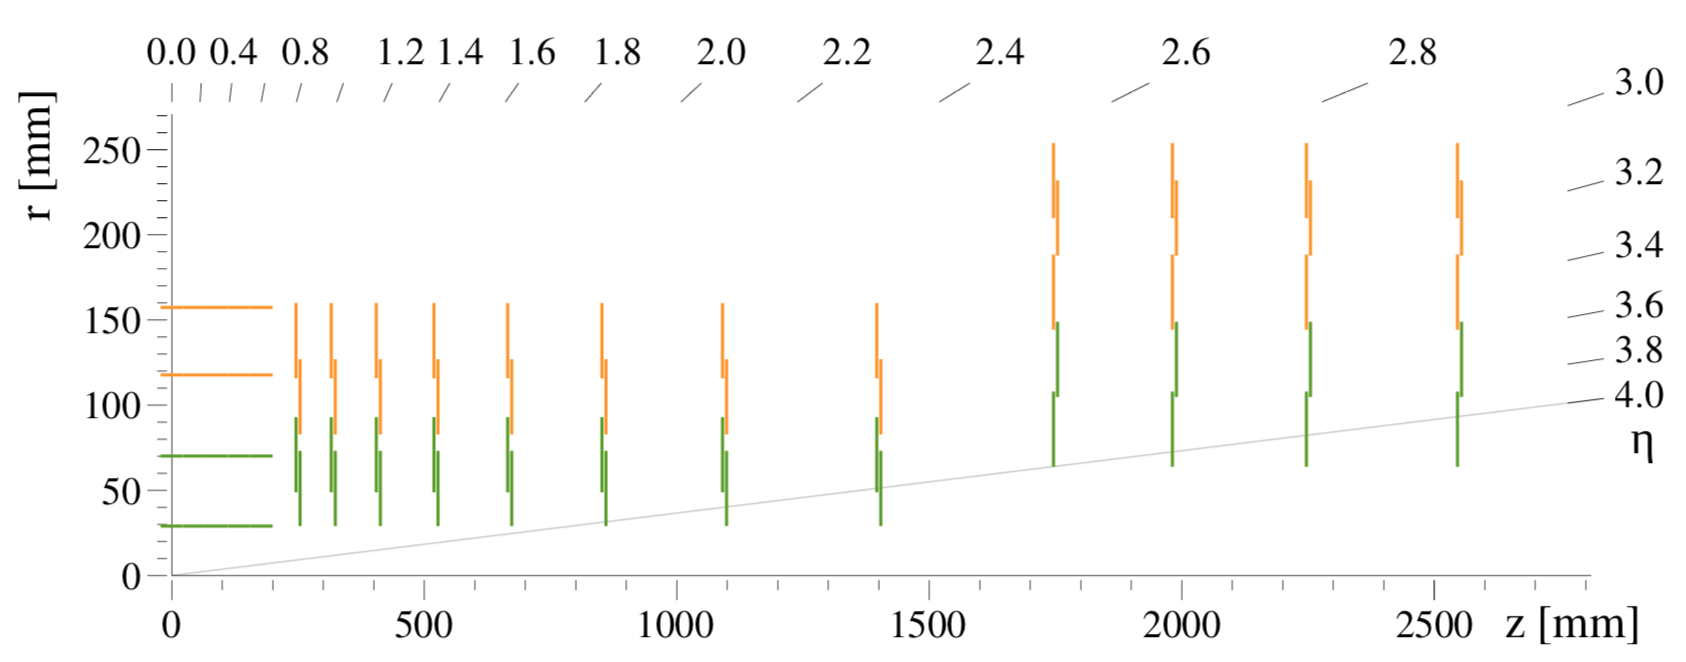
\includegraphics[width=0.63\textwidth]{figs/phase2_inner_tracker_geometry_lowres.png}
\centering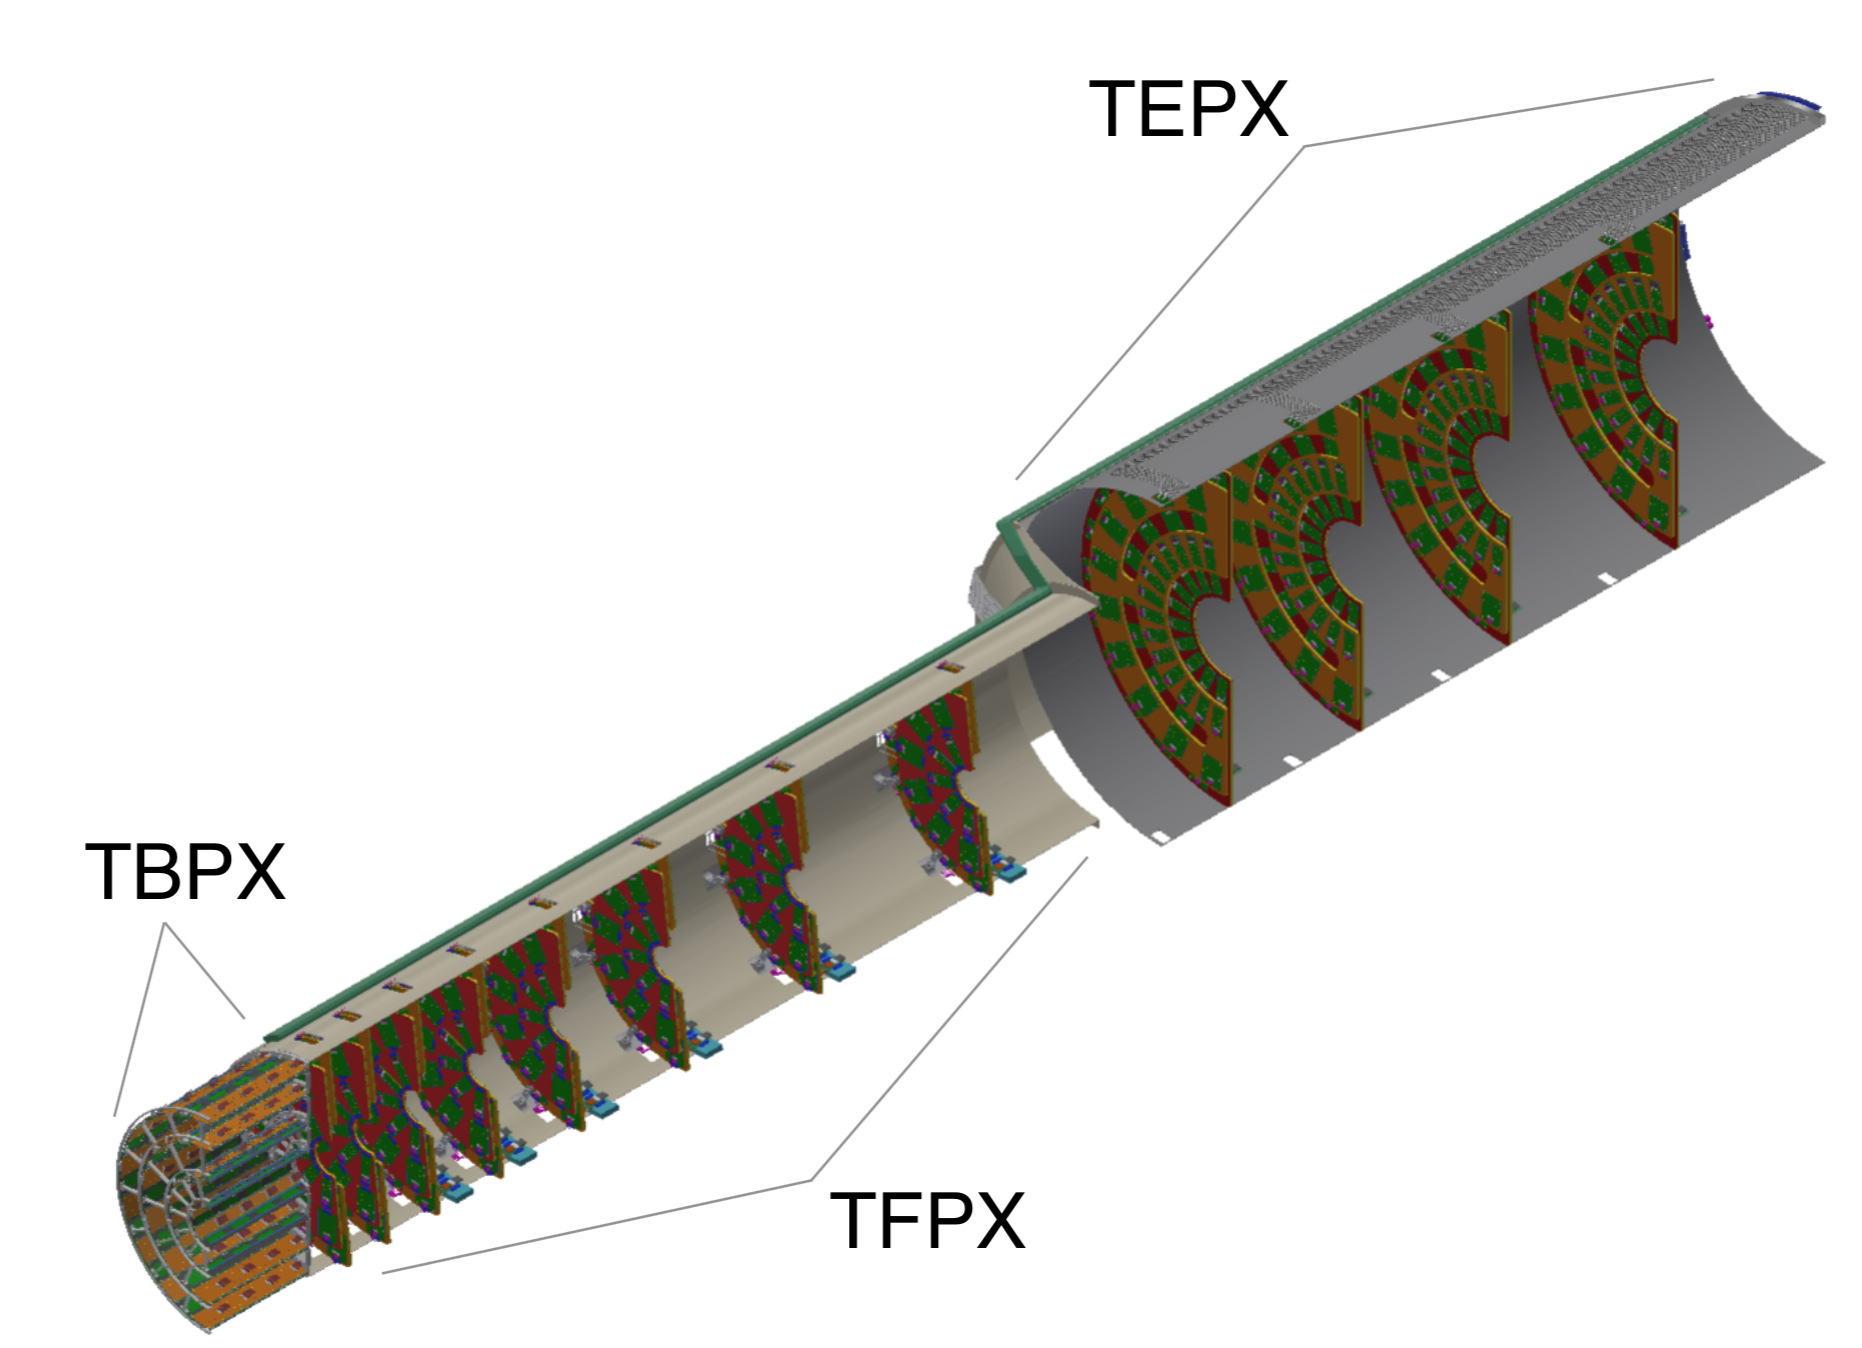
\includegraphics[width=0.35\textwidth]{figs/phsae2_inner_tracker_3D.png}
\caption{\label{fig:TFPX} Left: Geometry of the Phase~2 CMS Inner Tracker shown in $Rz$ projection. Right: A 3D drawing of the Inner Tracker with the major subdivisions indicated.}
\end{figure}

The UNL HEP group will produce modules for TFPX, along with Purdue and CUA.  UNL site setup started last summer, and during the next three years we will finish preparation of our site for module production while participating in the ongoing R\&D of the module design. Module preproduction and the start of production will happen within these years, as described below.

\paragraph{Production scheme and UNL site preparation}

UNL is expected to produce about 900 TFPX modules. Each  has three major components (see Fig.~\ref{fig:TFPXmodule} (left)): the silicon sensor layer, the layer with several RD53A readout chips superimposed on the 50x50~$\mu$m pixels of the sensor, and the high density interconnect (HDI). Additional components for mechanical support, such as spacers, are possible. Each production site will receive ``bare modules'' of sensors bump-bonded to the chips by a commercial contractor as well as HDIs and other parts. The module production procedure, perfected at UNL during the production of the Phase~1 Pixel Detector, remains the same with three main stages: a) gluing affixes HDIs to the bare modules in an automated procedure that uses a computer-driven robotic gantry; b) wirebonding makes 400-800 electrical connections per module and with a high-end automatic wirebonding machine; c) encapsulating covers the wirebonds with a silicone elastomer on the gantry. Other steps of the  procedure include gluing of spacers, curing of the encapsulant in an oven, visual, electric, and mechanical quality control at different production stages, and final module quality-tier assessment. After introduction of CUA as the new production site, part of UNL equipment was transferred there, and will be re-acquired as described below. Among the critical items, the F\&K Delvotec G5 64000 wirebonder remains at UNL.
%All of the above steps of production had worked perfectly at UNL.  Since then, the F\&K Delvotec G5 64000 wirebonder has remained at UNL while the gantry has been transferred to CUA; this will be replaced using project funds.

\begin{figure}
\centering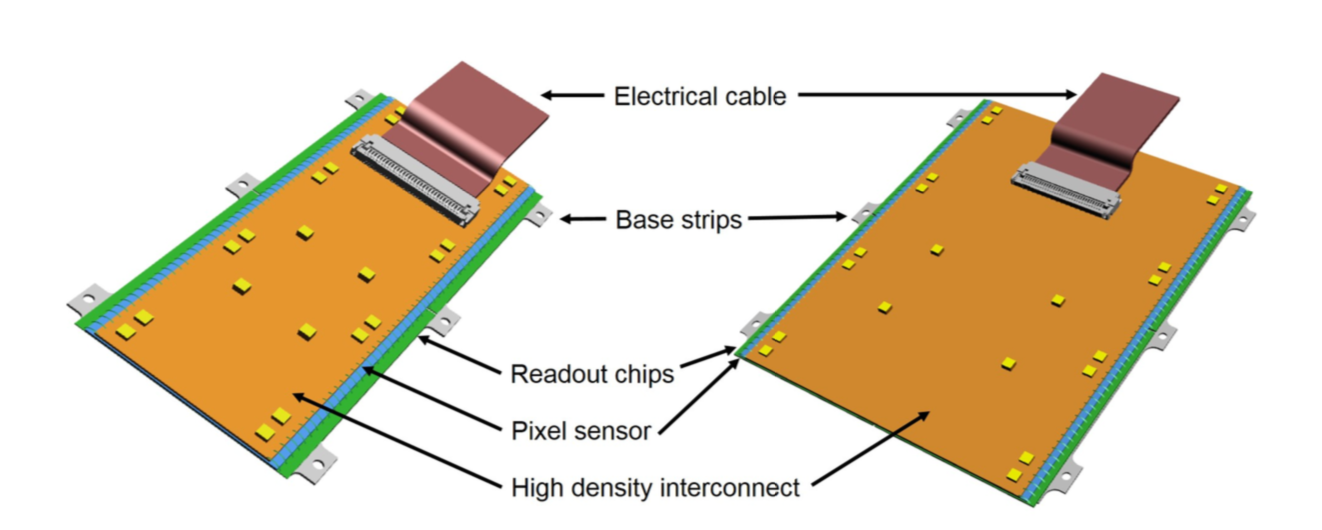
\includegraphics[width=0.43\textwidth]{figs/phase2_pixel_module_lowres.png}
\centering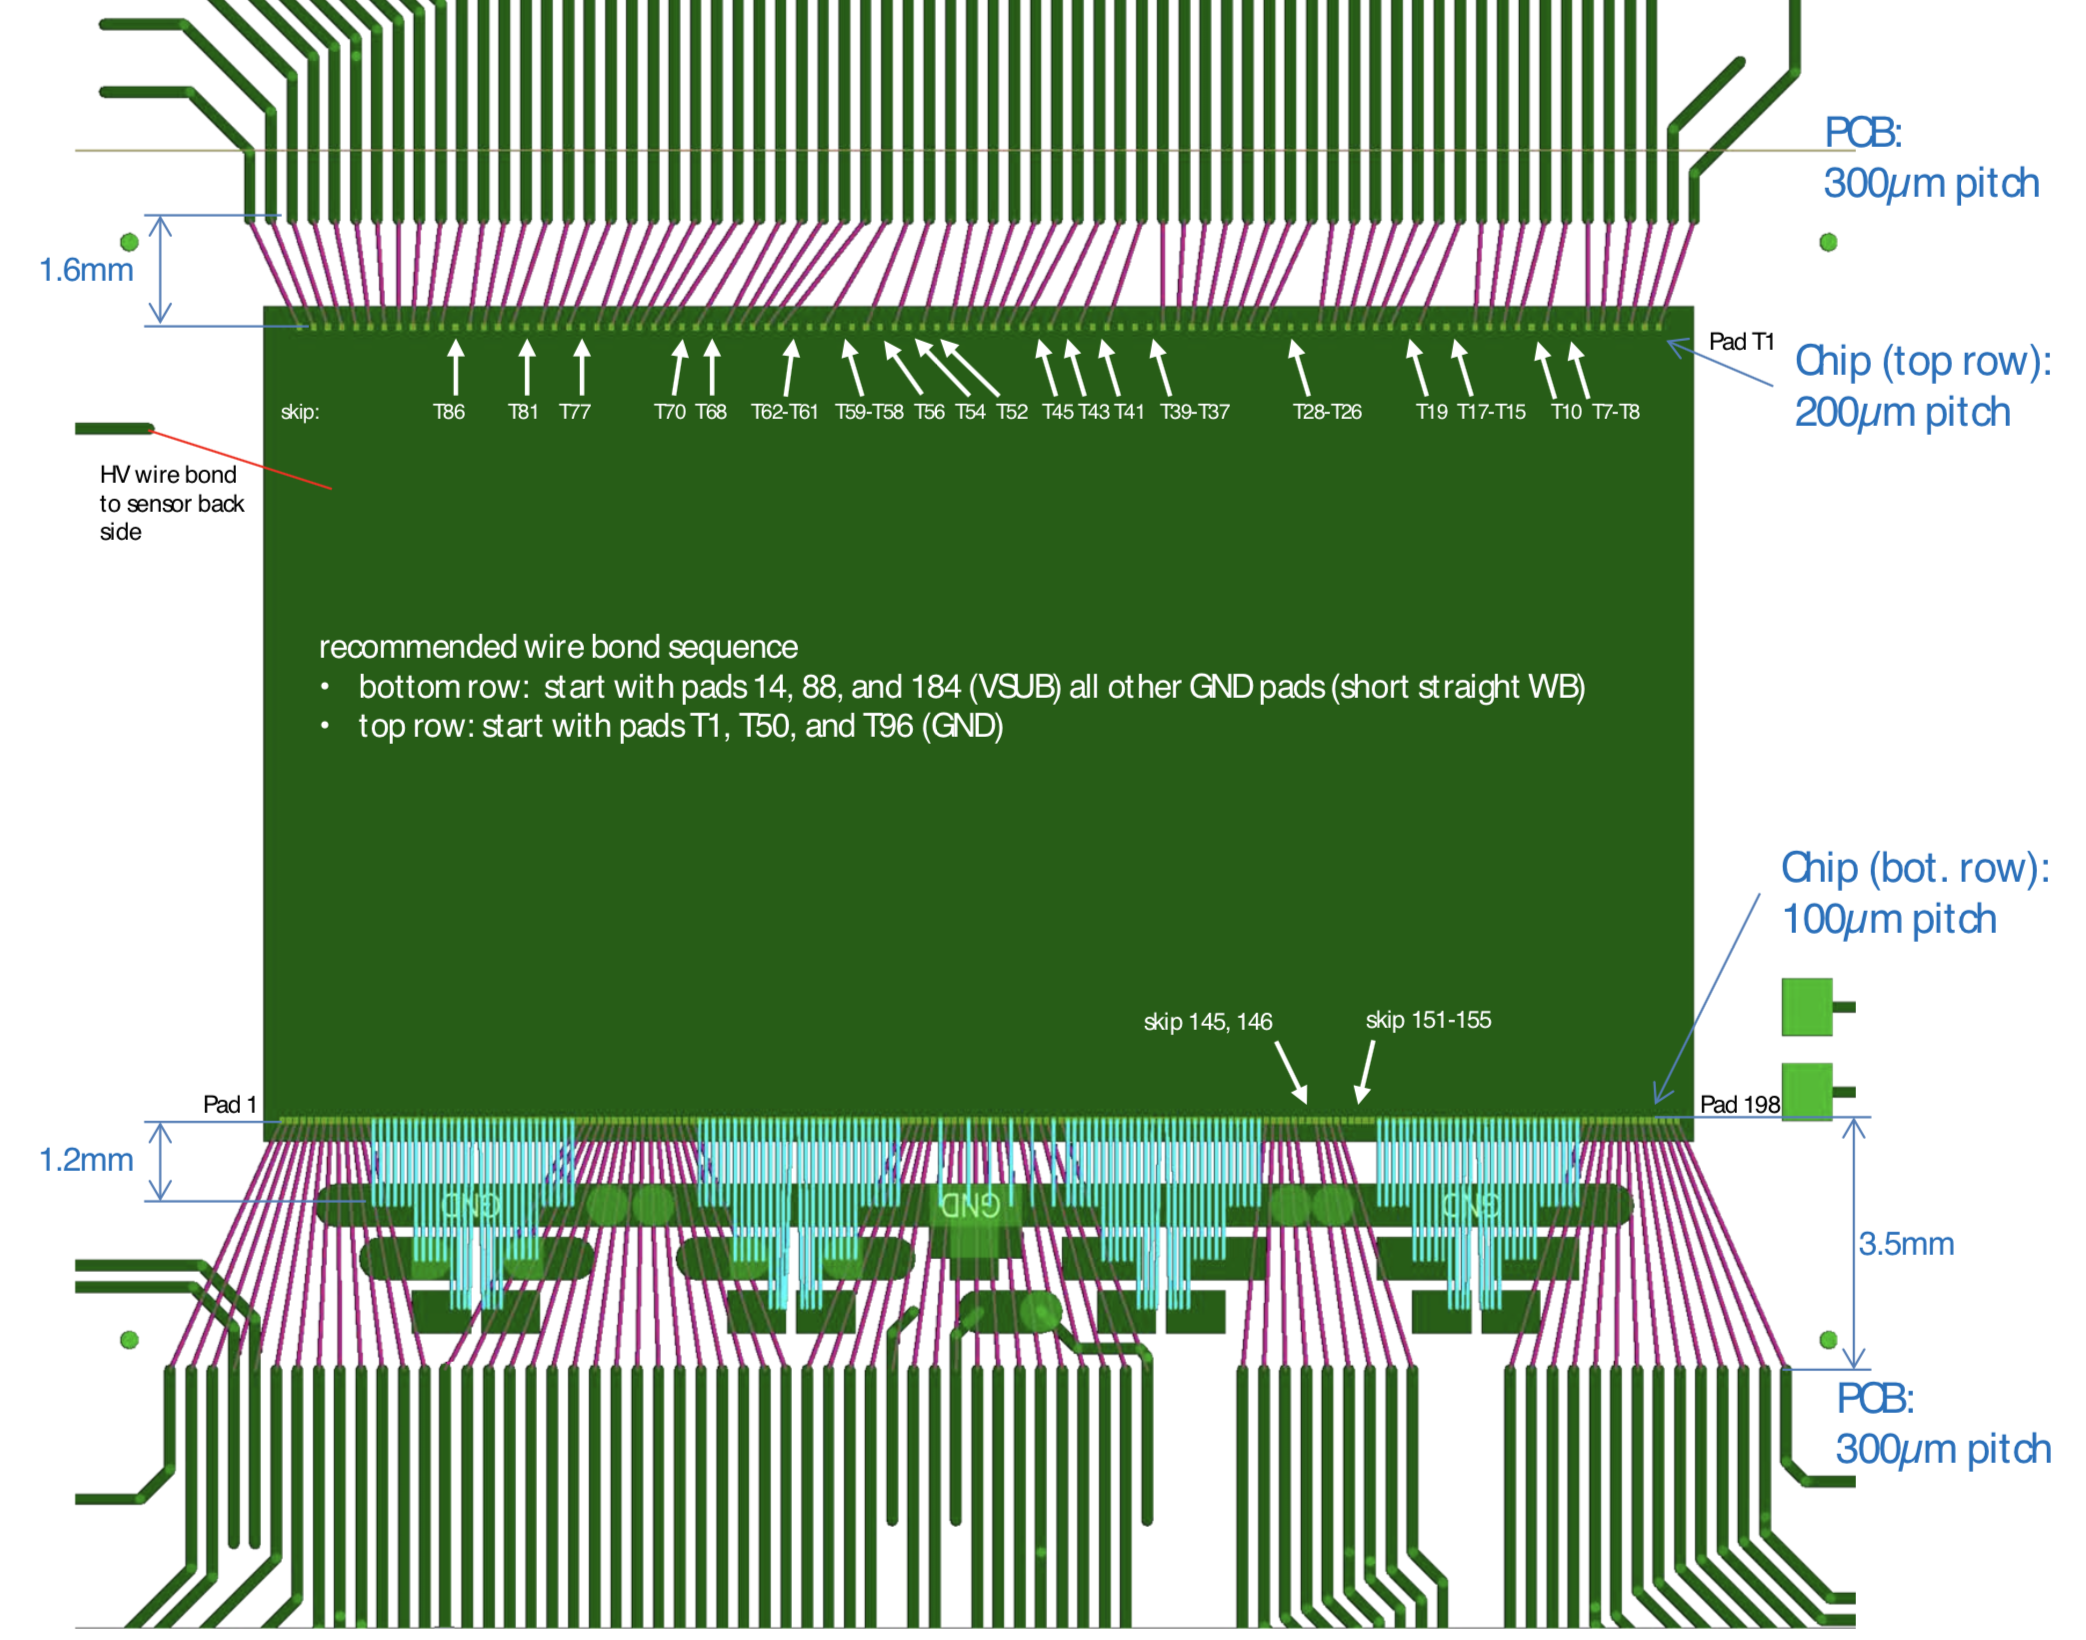
\includegraphics[width=0.30\textwidth]{figs/RD53A_wirebonding_diagram.png}
\centering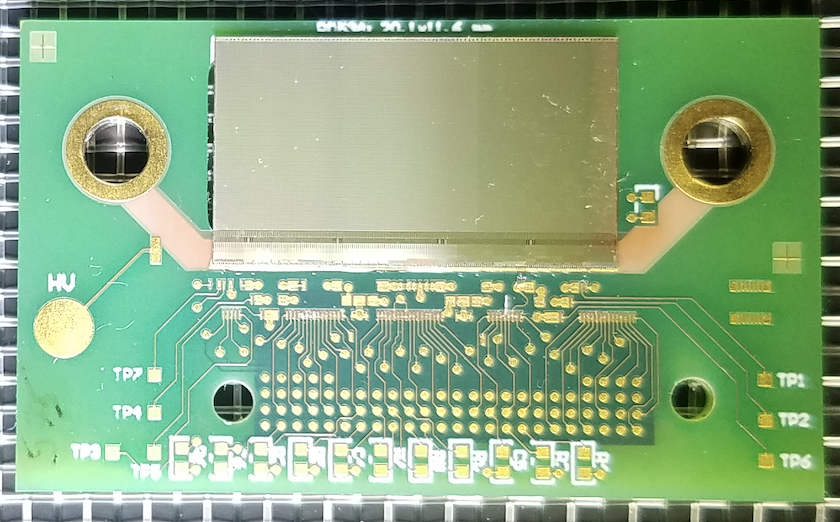
\includegraphics[width=0.25\textwidth]{figs/RD53A_bonded_chip.png}
\caption{\label{fig:TFPXmodule} Left: Conceptual view of a TFPX module with 1x2 and 2x2 readout chip layout. Center: wirebonding diagram for the RD53A chip. Right: prototype RD53A bonded to a PCB at UNL.}
\end{figure}

%%% Text below is duplicating the content of the "Personnel..."
%%% and is thus removed from here.
%At UNL, Kravchenko, along with a postdoc and the graduate students stationed at UNL, will lead project. Golf, who is submitting a separate concurrent proposal that focuses more on the MTD component of the Phase~2 upgrade, is also involved in TFPX as module production for both subdetectors is similar and the equipment will be shared. Claes and Snow will contribute to some of the tasks. 

Presently we are recommissioning the wirebonder, recovering the skills of programming it for complex bonding patterns, and  reestablishing the clean room operation.
The robotic gantry, critical to production, will be purchased with funds made available by the U.S.~CMS upgrade project and commissioned at UNL.  
%While the gantry can move and position its head with the accuracy of 10 microns or better, it comes ``bare''; 
The new gantry will coma ``bare'': custom tools need to be designed and made for each production process. The planned tooling includes pick-up tools to grab objects (vacuum-operated and mechanical), vacuum chucks to hold modules and their components, glue stamps, custom weights, glue syringe with vacuum control, positioning video cameras, and others. As for the Phase~1 gantry, the tools will be built by the UNL Physics Instrument Shop. Control software will be written for the new equipment. We will use Labview running on a PC that controls movements of the gantry, controls vacuum lines, and does positioning and fiducial calibration with video cameras. The setup will also include a manifold that supplies vacuum for various gantry tools and chucks controlled by the software through a voltage controller (planned as a compactDAQ from National Instruments). Several other stations will need to be set up, including a visual and mechanical test station, with a microscope and wirebonding pull test capability, and an electric/digital test station.  These will generally be built from parts provided by other institutes but will require assembly, automation and commissioning.

\paragraph{TFPX module R\&D, beam tests, module assessment}
While preparing for module production, we will continue our engagement in the R\&D on TFPX module design. Our group is now contributing to thermal behavior studies of the TFPX modules with Cornell and Purdue. We have wirebonded a set of ``thermal mockup modules'' designed to have 3~W power dissipation, just as the full modules, which will be used in coldbox tests and mockup-disks at our partners' sites. We wirebonded real RD53A prototype chips (see Fig.~\ref{fig:TFPXmodule} center, right) for the November 2018 beam tests at FNAL to assess the radiation resistance of production modules.  
Claes and Siado, now involved in beam tests of MTD subdetector modules, will be testing prototypes for TFPX at 2019 and 2020 beam tests until the chip and module design is fully settled. In this period, we will produce a number of modules with design variations for electrical, thermal, and mechanical studies.

The modules manufactured at UNL must be thoroughly tested before they are installed in the detector. While the most comprehensive tests will be done at UIC, UNL will perform a ``lite-test'' of new modules. The testing procedure and the test stands will be developed at FNAL and UIC during Sep. 2019 - Feb. 2020. Module production sites must participate in this development to understand the equipment, gain expertise with the chips, and ensure realistic choices for the lite-test at a production site. Claes and Siado, along with a UNL postdoc, will be part of this activity. It is expected that either Siado or the postdoc will spend several months at FNAL and UIC in the beginning of the period of this proposal, with travel support anticipated from the U.S.~CMS upgrade project or LPC visitors program.

\paragraph{Module preproduction and production}

Module preproduction and site commissioning will last 5-6 months. 
%While only a small number of modules will be produced, 
This will be an intense period of perfecting the production process, interacting with partners upstream (from where components come) and downstream (where modules go for testing), and learning how to quickly solve production problems. 
%%% Names are moved to the personnel part
%Kravchenko will coordinate preproduction and the postdoc will contribute significantly, up to 80\% of his or her time, during this period. 
Module production follows and will last 1.5 years, with the first half a year falling under the period of this proposal.  
%%% The names below also moved to the personnel section
%Production work will be distributed in a balanced way among the personnel including Kravchenko and Claes as coordinators, the postdoc, graduate and undergraduate students, and technicians from the Electronics and Instrument Shops, following the example of successful Phase~1 module production at UNL.

\paragraph{Timeline and personnel}

The described Phase~2 work requires significant personnel resources. Kravchenko will lead the TFPX effort at UNL in close collaboration with Golf who will focus on MTD and contrinute to TFPX. The concurrent proposal by Golf reflects the synergy between the module production for MTD and TFPX as the steps are similar and equipment is shared. Claes will take charge of FNAL test beams and module testing activities. A postdoc stationed at UNL will have major responsibilities including setting up all production stations on schedule, and preparing custom gantry tooling with the UNL Instrument Shop.
%, and becoming a wirebonding expert. 
Subsequently, the postdoc will see to successful module preproduction and production. Two or three graduate students will write the software for gantry and other equipment, and will maintain it through production. Fangmeier and Siado were major participants in  Phase~1 production software development, and will help the project by passing their expertise to the next generation. This project is an excellent opportunity to involve undergraduate researchers, as was done during Phase~1 production, when a number of undergraduates executed simpler projects of site preparation. The topics of several specific projects for undergraduates are already prepared.
%The first planned projects for undergraduates include, automatic control of an oven for curing encapsulated wirebonds using a simple electronics board with, e.g., a thermocouple and an Arduino chip that switches a power supply on and off, or video camera control for taking diagnostic photos of the modules. 
Finally,  wirebonding operation will be done by the UNL Electronics Shop technicians who participated in the Phase~1 production as well, with their time supported by the U.S.~CMS upgrade project.

The timeline of this project is driven by the schedule of the U.S.~CMS Phase~2 upgrade, with milestones listed in the table below.

\vspace{3mm}
\noindent
\begin{tabular}{l|l}
\hline
present - Apr 2020 & clean room recommissioning, equipment setup, wirebonding \\
        &  operations, R\&D and testbeam participation \\
Apr 2020 - May 2021 
         & major equipment (gantry, etc.) is provided by the project, gantry \\
         & custom tooling, software development, finish production preparation \\
Jun 2021 - Nov 2021
         & TFPX module preproduction, address any issues that arise \\
Dec 2021 - Jul 2023 
         &  TFPX module production (900 modules planned) \\
\hline
\end{tabular}

\subsection{CMS Detector Operations}
An experimental apparatus as complex as the CMS Detector requires a large crew of experts taking care of it 24/7 online and offline. The experiment has a team of shifters responsible for the central detector systems, a team Shift Leader, and several Run Field Managers who oversee multiple shift crews over longer time periods. 
%Each subdetector also has dedicated experts on call. 
All CMS signing authors are expected to participate in data-taking activities, but the UNL group will go beyond simple shift duties, as members of the group stationed at CERN will contribute at key points of detector operations.  Our postdocs and sometimes even graduate students routinely serve as Run Field Managers, a position near the top of data taking coordination hierarchy, and in a position of a Shift Leader.
%, and as experts-on-call for the CMS pixel detector operation. 
All UNL graduate students stationed at CERN will be expected to take the most critical central shifts, managing the Data Acquisition, Trigger and Data Quality Monitor systems. While the operations during 2019 and the first half of 2020 are expected to be on the light side, experts at CERN will still be needed to keep the detector running the experiment in the cosmic ray mode. In the second half of 2020 we expect rapid ramp-up and recommissioning of the detector and then intense activity as Run~3 commences. 
